\chapter{硬件设计实现}\label{chap:hardware}


\section{Xilinx FPGA 设计套件}

在上一章节中提到,本设计选用的芯片信号为 XC7Z045-2FFG900I,其为著名的 FPGA 供应厂商 Xilinx 研发。Xilinx 提供了非常完整的可编程逻辑开发软件工具链,及 Vivado 设计套件,使用该套件可以将我们的 Verilog 文件封装成知识产权 IP,进行硬件电路的仿真,生成比特流与硬件描述文件等功能。使用 ZYNQ 器件,也需要我们在 Vivado 的 BlockDesign 页面中分配 ARM 处理器使用到的资源。除此之外,Vivado 设计套件还包括了开发 ARM 裸机的 Vivado SDK、能够基于 LLVM 将 C$\backslash$C++ 程序转换为底层逻辑电路的 Vivado HLS 等应用。

本章节将说明如何使用 Vivado 设计套件完成 NVDLA IP 的打包,Block Design 设计,查看资源利用、时序、功耗等报告,最后生成比特流文件与硬件描述文件。 

\section{NVDLA IP 生成描述}

这一小节将详细介绍如何修改 NVDLA 的配置文件,以及根据配置文件生成 NVDLA 的 RTL 代码,并将 NVDLA 的接口进行封装,打包成 IP。

总的来说,生成 NVDLA 的 RTL 代码有两个路径,其一是英伟达官方提供的 hw 项目,可以根据预先定义好的 spec 文件生成,但是这个工作流程需要预先构建好官方提供的 \emph{make} 工具,该工具又依赖 GCC、Java、Perl、Verilator、Python 等,稍显复杂。第二条路径是使用一名由伯克利大学的研究生使用 Chisel 语言编写的 NVDLA 项目,其也是可以生成 RTL 代码的,但是由 Chisel 生成的 RTL 代码会被压缩在一个文件之内,NVDLA 的代码输出高达数万行,不利于阅读与分析。

综合以上,本文使用 \emph{make} 进行 RTL 生成,并且使用 Docker 容器技术分离环境解决 \emph{make} 软件依赖过复杂的问题。

\subsection{基于 \emph{make} 的 RTL 生成}

为了能够在不污染主机环境的情况下构建 \emph{make} 工具,本设计使用 Docker 容器技术搭建软件环境,基于 Ubuntu:16.04 容器,安装好如下环境:

\begin{itemize}
    \item GCC 4.8.5
    \item OpenJDK 1.8.0
    \item SystemC 2.3.0
    \item Python 2.7.12
    \item VCS 2016.06
    \item Verilator 3.912
    \item Clang 3.8.0
\end{itemize}

安装好环境之后,我们可以通过新建一个 spec 文件来修改NVDLA的配置。例如通过定义宏 FEATURE\_DATA\_TYPE\_INT8 可以指定 Feature Map 的数据格式为 INT8;通过定义宏 WINOGRAD\_DISABLE 来关闭 WINOGRAD 卷积电路。本设计采用的是官方提供的最小配置,及使用 small.spec 文件。

有关 small.spec 的详细内容详见附录,在使用 \emph{tmake} 之前,我们还需要在根目录通过 \emph{make} 命令选择 small.spec 为配置文件,并输入安装的软件生态的可执行文件路径,该 \emph{make} 命令最终会生成一个 tree.make 的文件,\emph{tmake} 工具的本质是根据与现实先定义好的宏,将模板文件夹 vmod 里的 Verilog 代码进行文本预处理,将不需要的文本删除输出。

\lstset{language=Bash}
\begin{lstlisting}
./tools/bin/tmake -build vmod
\end{lstlisting}

执行完该命令之后,可以被综合的 Verilog 代码将会被存放在 out 文件夹下,此时已经可以通过 Vivado 导入文件夹解析依赖,但是由于 NVDLA 是面向 ASIC 设计,内部 RAM 的 Verilog 代码是结构级描述,这意味着在例化 RAM 的时候会消耗大量 FPGA 片上珍贵的 LUT 资源,所以在导入之前需要将所有的 RAM 替换成 FPGA 内部的 Block RAM。

\subsection{替换 Block RAM}

替换 RAM 的方法也有两种,其一是例化 Vivado 设计免费提供的 BRAM Controller IP,但是 NVDLA 使用到的 RAM IP 过于繁杂,替换工作量巨大,第二是使用官方提供的行为级描述的 Verilog RAM 模块代码,本设计使用第二种。

具体步骤为,将原本的 \emph{vmod/rams/synth} 文件夹删除,在 Vivado 导入文件夹的时候,使用 \emph{vmod/rams/fpga} 文件夹。

\subsection{csb2apb}

从 Vivado 导入 vmod 文件夹之后,NVDLA 的顶层模块文件为 \emph{NV\_nvdla.v} ,但是本设计还做了另一层封装,使用英伟达官方提供的 csb2apb 电路,将原本的 CSB 总线转化为 APB 总线,这样能够方便我们在 Vivado 设计中使用内存映射读写 NVDLA 的寄存器。

在 Vivado 设计中,新建一个 wrapper 文件,命名为 \emph{Nv\_nvdla\_wrapper.v} ,详细内容见附录。在其中例化了 \emph{NV\_nvdla} 与 \emph{NV\_NVDLA\_apb2csb} 两个电路,并且补全了 AXI 总线与 APB 总线缺失的信号线,方便在后期 IP Package 阶段自动推导封装总线接口。

\subsection{关闭 Clock Gating}

再次由于 NVDLA 是面向ASIC设计,内部的 RAM 在例化的时候默认有 Clock Gating 电路用来降低功耗,但是 FPGA 的时钟树是设计好的,不需要该电路,否则可能会因为 Clock Buf资源不够导致布线过不去,在 Vivado 的全局变量里,添加如下几个 Global Define,关闭不必要的电路:

\begin{itemize}
    \item VLIB\_BYPASS\_POWER\_CG
    \item NV\_FPGA\_FIFOGEN
    \item FIFOGEN\_MASTER\_CLK\_GATING\_DISABLED
    \item FPGA
    \item SYNTHESIS
\end{itemize}


\subsection{封装AXI、APB总线}

为了方便之后 BlockDesign 中连线,也为了给 APB 总线挂上 Address Block,在 IP Package 阶段,我们需要 AXI 和 APB 总线进行包装,由于先前已经补全的信号线,这里我们让 Vivado 自动推导,包装完成后的 IP 核如图~\ref{fig:NVDLA Wrapper}所示。

\begin{figure}[!htbp]
    \centering
    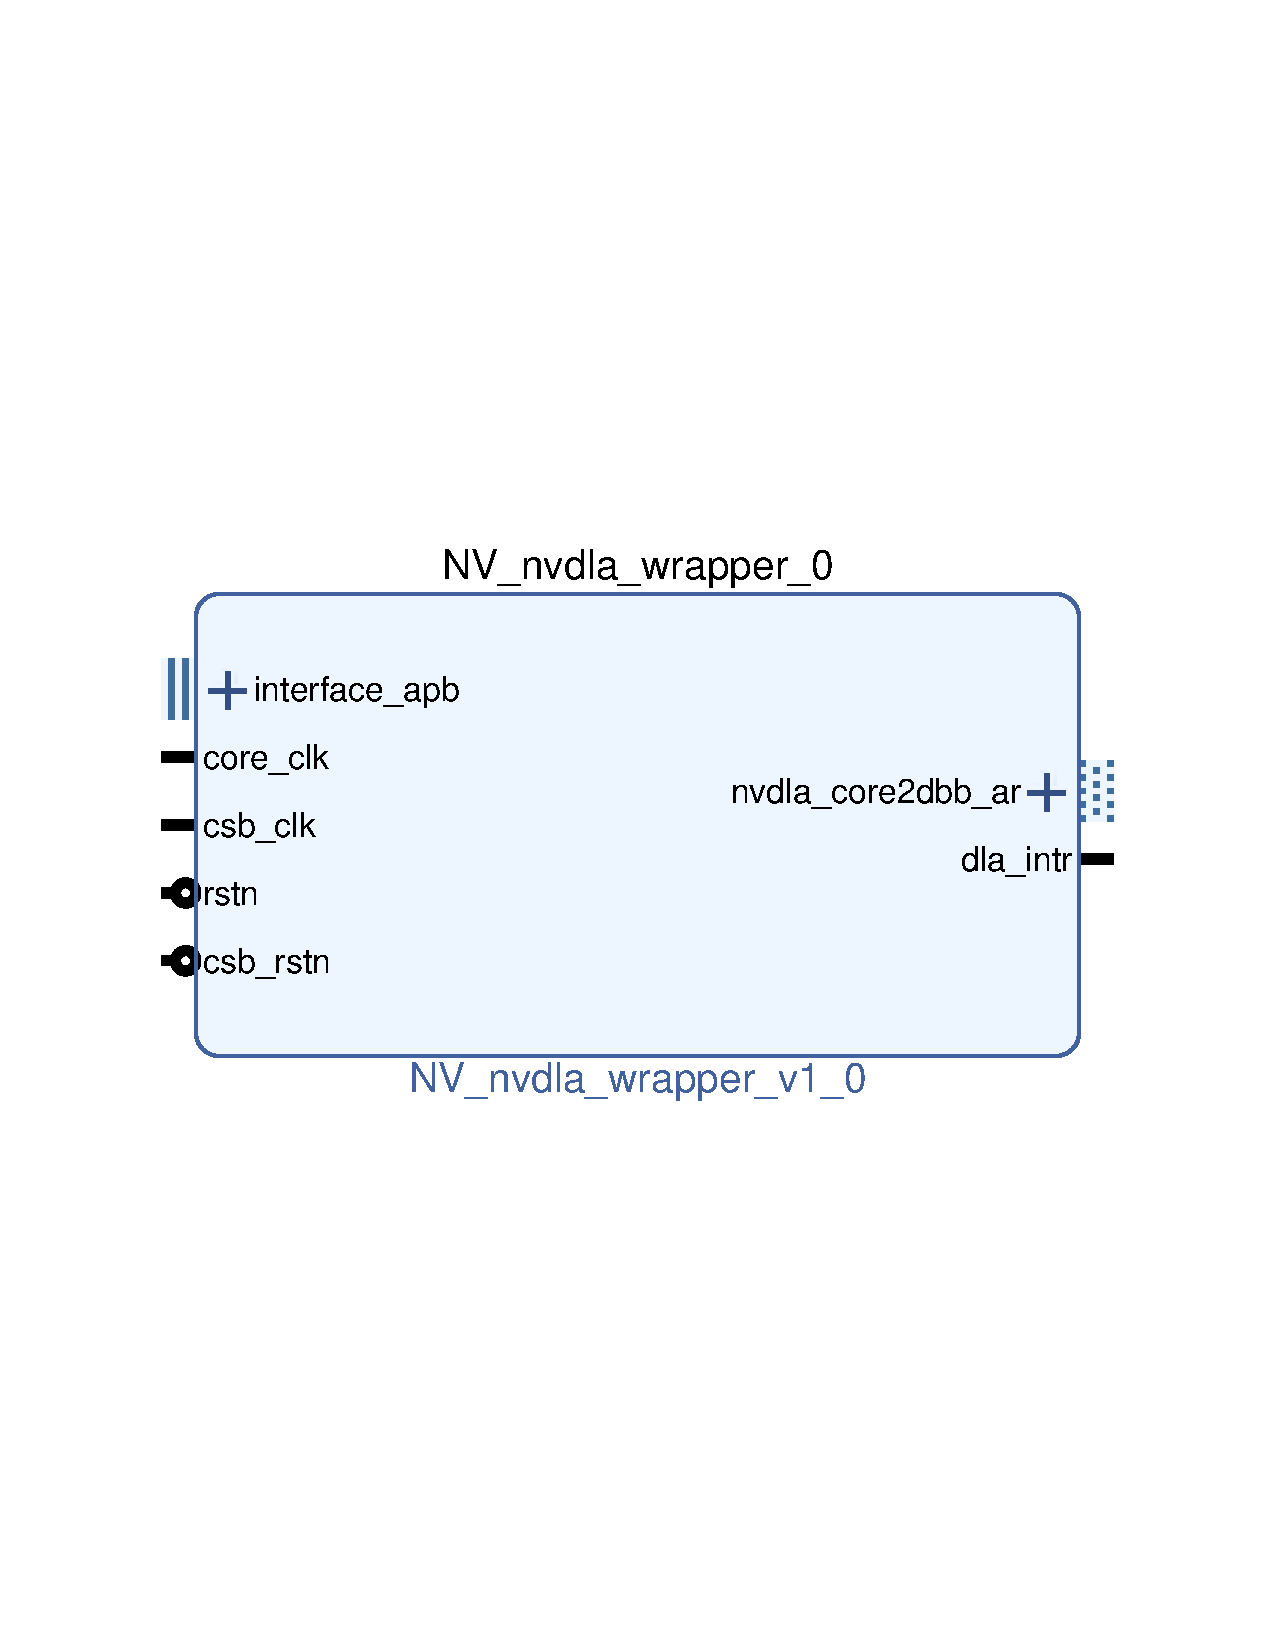
\includegraphics[width=0.9\textwidth]{dla_wrapper}
    \caption{NVDLA Wrapper IP}
    \label{fig:NVDLA Wrapper}
\end{figure}

\subsection{增加 Address Block}

在 IP Package 阶段,AXI 的 Memory Block 会自行分配,这样在进行 Block Design 的时候 Vivado 会自动分配地址完成内存映射。但是 APB 总线的 Memory Block 需要自行添加,在本设计中,为 APB 总线分配了 4KB 大小的寻址空间。

\section{Top Block Design 设计}

在我们的主工程中导入已经打包好的 NVDLA IP,并引入 APB to AXI Bridge、AXI Smart Connect、ZYNQ 7000+ 等其他知识产权 IP,他们的连线关系如图~\ref{fig:Block Design Connect}所示。

\begin{figure}[!htbp]
    \centering
    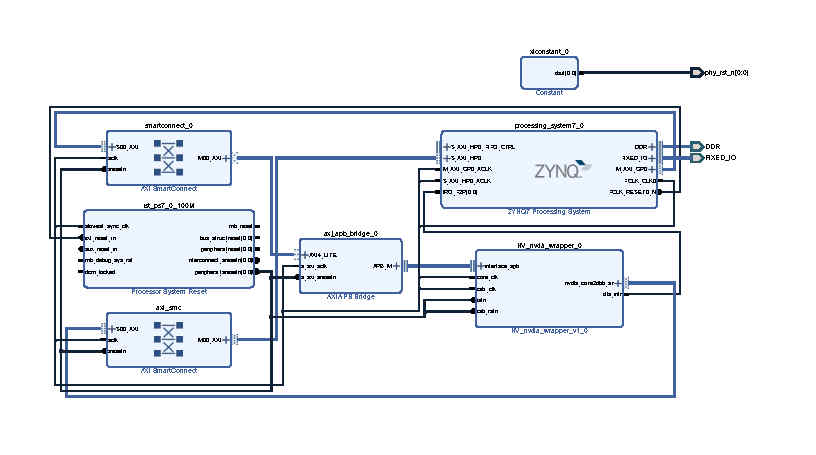
\includegraphics[width=0.9\textwidth]{nvsmall}
    \caption{Block Design Connect}
    \label{fig:Block Design Connect}
\end{figure}

\subsection{APB to AXI Bridge}

使用 APB to AXI Bridge 可以把 APB 总线协议转化为 AXI 总线协议,这样方便我们使用 Vivado 内部的 Connect IP 自动做内存映射。

\subsection{AXI Smart Connect}

Axi Smart Connect 的作用是用来自动配置 AXI 设备的内存映射,与 Axi InterConnect 的作用是一样的,但是 Smart Connect 更紧密的嵌入到了 Vivado 内部,不需要用户太多的干涉。

在本设计中用到了两个 Smart Connect ,其中一个是将 ZYNQ 的 AXI Master 接入了 NVDLA 的控制总线,以便通过内存映射机制读写 NVDLA 的寄存器;另一个将 NVDLA 的主内存接口接入了 ZYNQ 的 AXI Slave,这样就可以 NVDLA 就可以访问挂在在 ARM 侧的 DDR 存储,与处理器共用内存,处理器可以通过硬件 DMA 搬移数据,加快访存速度。

\subsection{ZYNQ 7000+ AP SOC}

ZYNQ 7000+ 的 IP 如图~\ref{fig:ZYNQ 7000+}所示,在本设计中,启用了如下资源:

\begin{itemize}
    \item 以太网接口(Ethernet0),在软件设计章节,本文将在 SOC 上构建 Linux 操作系统,使能以太网接口可以使板卡通过以太网线访问互联网,方便开发与调试。
    \item SD卡接口(SD0),用来存放 Linux 操作系统的 BOOT 与 IMAGE 文件。
    \item 串口(UART0),用来实现串口终端,方便调试。
    \item FCLK\_CLK0,输出时钟,该时钟可以作为可编程逻辑端的输入时钟,这样不需要额外对片外的时钟输入做约束,在本设计中该时钟取 100Mhz,有关 100Mhz 的取值,详见综合报告。
\end{itemize}

\begin{figure}[!htbp]
    \centering
    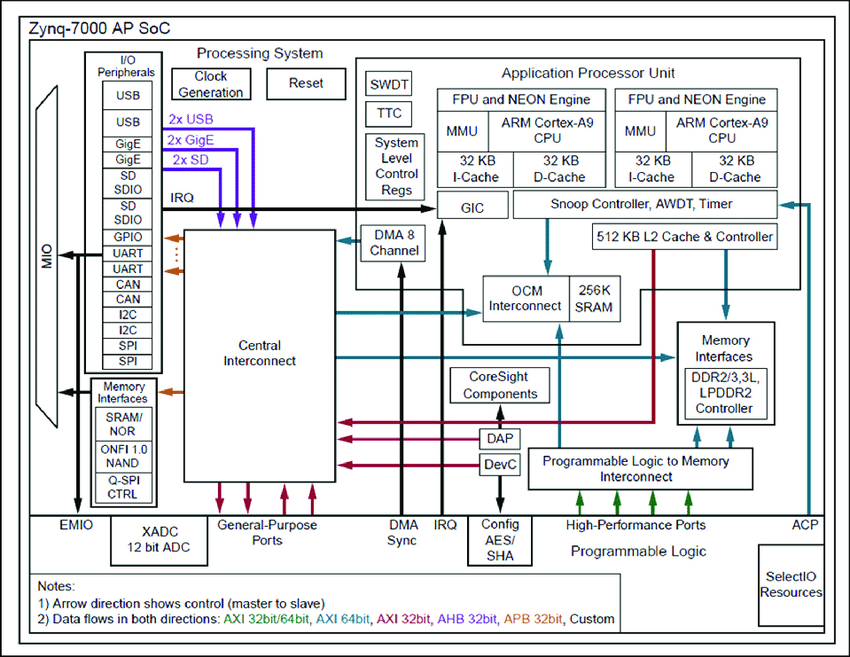
\includegraphics[width=0.9\textwidth]{ZYNQ 7000.png}
    \caption{ZYNQ 7000+ block diagram}
    \label{fig:ZYNQ 7000+}
\end{figure}

\section{综合}

硬件设计完成之后,首先需要经过综合,在这一小节,我们分别列出资源利用率报告,Timing 报告与功耗报告。

\subsection{资源利用率报告}

在本章节,我们主要分析 Timing 报告得出对于 NVDLA 能够给与的最大输入时钟,这需要我们更改输入时钟来反复综合,在这个过程中硬件的资源利用率是不会变化的,所以我们首先给出硬件资源利用率报告,其一般也是我们再进行 FPGA 设计的时候首先需要查看的报告。

\begin{table}[!htbp]
    \caption{资源利用率报告}
    \label{tab:Resource Report}
    \centering
    \footnotesize% fontsize
    \setlength{\tabcolsep}{4pt}% column separation
    \renewcommand{\arraystretch}{1.2}%row space 
    \begin{tabular}{llll}
        \toprule
        \textbf{RESOURCE} & \textbf{UTILIZATION} & \textbf{AVAILABLE} & \textbf{Utilization \%} \\
        \midrule
        LUT               & 80959                & 274080             & 29,54                   \\
        LUTRAM            & 689                  & 144000             & 0,48                    \\
        FF                & 94802                & 548160             & 17,29                   \\
        BRAM              & 100,50               & 912                & 11,02                   \\
        DSP               & 32                   & 2520               & 1,27                    \\
        BUFG              & 1                    & 404                & 0,25                    \\
        \bottomrule                   
    \end{tabular}
\end{table}

\subsection{Timing 报告}


\subsection{功耗报告}

\section{实现}

实现是紧接着综合的下一个步骤,在这个过程中会进行布局布线。综合后生成的门级网表只是表示了门与门之前虚拟的连接关系,并没有规定每个门的位置以及连线的长度等,布局布线就是将门级网表中的门的位置与连线信息确定下来的过程。

所谓布局,及是将每一个门映射到 CLB 的过程;所谓布线,是利用FPGA中丰富的布线资源将 CLB 根据逻辑关系连接在一起的过程。

\section{Bitstream 与 hdf 文件生成}

最后,生成 Bitstream,有了 Bitstream 就可以将设计的数字电路烧录到 FPGA 板卡中去,但是本设计仅将 Bitstream 烧录到板卡中去是没有效果的。在下一章节,我们需要在 ARM 上构建 Linux 系统,需要我们生成 HDF 硬件描述文件,为了生成 HDF 文件,需要使用到 Vivado SDK,在 Vivado 中选择 Export Hardware,则 HDF 文件会在 SDK 目录下自动生成。








